\ChapterImageStar[cap:revisionLiteratura]{Revisión sistemática de la literatura}{./images/fondo.png}\label{cap:revisionLiteratura}
% !TODO Insertar Taxonomía
\mbox{}\\
\section{Construcción de la bitácora}

Con el propósito de establecer una base teórica sólida para el desarrollo de una notación de modelado de infraestructura de~\TI~(\NDITI) y de garantizar decisiones fundamentadas durante su diseño y validación, se llevó a cabo una revisión exhaustiva de la literatura relacionada con las principales notaciones y marcos de modelado empleados en el ámbito de la infraestructura de~\TI. Este proceso se desarrolló en múltiples etapas, orientadas a identificar las fortalezas, limitaciones y oportunidades de estandarización presentes en cada enfoque analizado.

\subsection{Planeación}

Esta fase tuvo como propósito establecer los lineamientos generales del estudio de mapeo sistemático (\SMS), tomando como referencia la metodología propuesta por \cite{Sepulveda2021}.
esta etapa se definieron las metas del estudio (ver cuadro~\ref{tab:metas}), junto con las preguntas de investigación (ver cuadro~\ref{tab:preguntas}) y las métricas de evaluación (ver cuadro~\ref{tab:metricas})que orientaron el proceso de análisis. Para garantizar la coherencia metodológica, se adoptó el enfoque
Objetivo-Pregunta-Métrica (\textit{goal-question-metric}, GQM) que permite vincular de manera estructurada las metas del estudio con los indicadores y evidencias obtenidas.

\subsubsection{Definición de metas para el \SMS}

% Tabla METAS DEL SMS
\begin{table}[H]
	\centering
	\renewcommand{\arraystretch}{1.2} % Espaciado reducido
	\fontsize{9pt}{10pt}\selectfont % Tamaño de fuente 8pt
	\begin{tabular}{|p{1.5cm}|p{12.5cm}|}  % Total: 14cm
		\hline
		\textbf{Meta} & \textbf{Descripción}                                                                                                                                                                                                                                                                                                                                         \\ \hline
		G1            & Clasificar los trabajos relacionados con metodologías, tecnologías, modelos y frameworks relacionados con~\NDITI~que satisfagan las necesidades identificadas en el contexto de computación, networking y los casos de negocios. \\ \hline
		G2            & Identificar la tendencia de uso de herramientas tecnológicas en los trabajos relacionados con una notación de diseño en el contexto de diversas áreas de infraestructura de~\TI.                                                                                                                                                     \\ \hline
	\end{tabular}
	\caption{Definición de metas del SMS}
	\label{tab:metas}
\end{table}


\subsubsection{Definición de preguntas de investigación}\label{subsubsec:RQ-def}
%TABLA GOAL VS Preguntas
\begin{table}[H]
	\centering
	\renewcommand{\arraystretch}{1.2} % Espaciado reducido
	\fontsize{9pt}{10pt}\selectfont % Tamaño de fuente 8pt
	\begin{tabular}{|p{0.7cm}|p{1.3cm}|p{5.5cm}|p{6cm}|} % Total: 14cm
		\hline
		\textbf{Meta}                                                                                                                                                                                                                                                                                                                                    & \textbf{Pregunta} & \textbf{Descripción} & \textbf{Motivación}        \\ \hline

		G1                                                                                                                                                                                                                                                                                                                                               & Q1                &
		\textit{¿Cuáles son los trabajos relacionados con metodologías enfocadas a una notación de diseño de infraestructura de~\TI~que dan solución a necesidades identificadas en el contexto de computación, networking y los casos de negocios?} &
		Las notaciones de diseño de infraestructura de~\TI~permiten modular esquemas según diversos criterios específicos. Sin embargo, de establecer criterios unificados que orienten dichas notaciones, existiría una facilidad en la construcción y comprensión de los modelos realizados. \\ \hline

		G2                                                                                                                                                                                                                                                                                                                                               & Q2                &
		\textit{¿Cuáles son los trabajos relacionados con herramientas tecnológicas de mayor tendencia asociados a notaciones de diseño en el contexto de la infraestructura de~\TI?}                                                                                                                                                                           &
		El estudio del impacto generado permite caracterizar de una manera más efectiva aquellas características fundamentales presentes en estas herramientas tecnológicas que optimizan el desarrollo de estos trabajos relacionados.                                                                                                                                                           \\ \hline
	\end{tabular}
	\caption{Definición de preguntas de investigación del SMS}
	\label{tab:preguntas}
\end{table}

\subsubsection{Definición de métricas}
%Tabla METRICAS
\begin{table}[H]
	\centering
	\renewcommand{\arraystretch}{1.2} % Menor espaciado entre filas
	\fontsize{9pt}{10pt}\selectfont % Tamaño de fuente 8pt
	\begin{tabular}{|c|p{13cm}|} % Total: 14cm
		\hline
		\textbf{Métrica} & \textbf{Descripción}                                                                                                                                                                                                                                                                                                                                                                                                                                                                                           \\ \hline
		M1               & Cantidad de trabajos relacionados a metodologías asociadas a notaciones de diseño de \TI. \\ \hline
		M2               & Cantidad de trabajos relacionados con herramientas asociadas a notaciones de diseño de \TI.                                                                                                                                                                                                                                                                                                                                                                                                                                                    \\ \hline
		M3               & Cantidad de trabajos relacionados con enfoques asociadas a notaciones de diseño de \TI.                                                                                                                                                                                                                                                                                                                                                                                                           \\ \hline
		M4               & Cantidad de trabajos relacionados con tendencias asociadas a notaciones de diseño de \TI.                                                                                                                                                                                                                                                                                                                                                                                                                 \\ \hline
	\end{tabular}
	\caption{Definición de métricas del SMS}
	\label{tab:metricas}
\end{table}


\newpage \section{Búsqueda de estudios}


Esta etapa comprendió las siguientes secciones:
\begin{enumerate}
	\item Estrategia de búsqueda, ya sea independiente o combinada;
	\item Identificación general de estudios;
	\item Revisión de estudios; y finalmente,
	\item Selección de estudios para incluir en el SMS.\@
\end{enumerate}

\subsection{Estrategia de búsqueda}

En esta etapa, el proceso de revisión combinó estrategias de búsqueda en bases de datos académicas con la técnica de búsqueda en bola de nieve (\textit{snowballing}), lo que permitió ampliar y enriquecer la recopilación de estudios relevantes para el mapeo sistemático. Esta metodología facilitó la identificación de investigaciones fundamentales que podrían no haber sido detectadas mediante una búsqueda convencional, garantizando así una visión más completa y representativa del estado del arte.

\subsection{Búsqueda en bases de datos}\label{subsec:busquedaBasesDatos}
Se seleccionaron las siguientes bases de datos para llevar a cabo el mapeo sistemático de estudios: ACM, IEEE Xplore, Springer, Taylor \& Francis y Science Direct. Estas fuentes fueron elegidas por su disponibilidad, relevancia y cobertura en el área de investigación, asegurando así la obtención de información actualizada y de calidad para el desarrollo del estudio.


\newpage
\subsubsection{Identificación de estudios mediante búsqueda en bases de datos}\label{subsubsec:identificacionEstudios}
En esta fase del proceso fue necesario definir un marco metodológico que facilitara la selección de las palabras clave más adecuadas para la búsqueda y clasificación de estudios dentro del mapeo sistemático. Con este propósito, se empleó el modelo PICOC (\textit{Population}, \textit{Intervention}, \textit{Comparator}, \textit{Outcome} y \textit{Context}) como guía estructural, permitiendo delimitar de manera precisa el alcance y los criterios de búsqueda en las bases de datos seleccionadas. El resultado de esta etapa se presenta en la tabla~\ref{table:modelo-picoc},donde se detallan los elementos definidos según cada componente del modelo.

% TABLA modelo PICOC: Población - Intervención - Comparación  - Salida - Contexto
\begin{table}[H]
	\centering
	\renewcommand{\arraystretch}{1.5} % Espaciado reducido
	\fontsize{9pt}{10pt}\selectfont % Tamaño de fuente 8pt
	\begin{tabular}{|c|p{12cm}|} % Total: 14cm
		\hline
		\textbf{Componente} & \textbf{Descripción}                                                                                                                                                                                                                                                                                                                                                                                                                                                                             \\ \hline

		Población           & Trabajos relacionados con metodologías, herramientas y tecnologías asociadas con notaciones de diseño de \TI.                                                  \\ \hline

		Intervención        & Identificación y clasificación de los trabajos de \NDITI según una taxonomía establecida. \\ \hline

		Comparación         &
		\textbf{1.} Comparar trabajos asociados con \NDITI's para determinar la tendencia de uso de metodologías, herramientas y/o  tecnologías.
		\textbf{2.} Verificar trabajos asociados con \NDITI's a través de la relación de estos con los parámetros de título, abstract y keywords.
		\textbf{3.} Analizar la tendencia de uso de \NDITI's mediante trabajos asociados al contexto de computación, networking y los casos de negocios.                                                                                                                                                                                                                                                                                                                                                                                                                                                                 \\ \hline
		Salida              & Taxonomía de clasificación de trabajos relacionados con NDITI según metodologías, herramientas y/o tecnologías.                       \\ \hline
		Contexto            & Computación, networking y casos de negocios con relación a metodologías, herramientas y tecnologías asociadas con notaciones de diseño de TI.                                                                                                                     \\ \hline
	\end{tabular}
	\caption{Modelo PICOC}
	\label{table:modelo-picoc}
\end{table}



%# TABLA Palabras clave indentificadas usando el modelo PICOC.
\begin{table}[H]
	\centering
	\renewcommand{\arraystretch}{1.4}
	\fontsize{8}{8}\selectfont
	\begin{tabular}{|p{3cm}|p{10.0cm}|}
		\hline
		\textbf{Categoría \hbox{PICOC}} & \textbf{Palabras clave} \\
		\hline
		Población                       &
		- Metodología \newline
		- Herramienta \newline
		- Tecnología \newline
		- Notaciones \newline
		- Diseño \newline
		- \TI 													   \\
		\hline
		Intervención                    &
		- Identificación  \newline
		- Clasificación  \newline
		- Taxonomia                                               \\
		\hline
		Criterios de aceptación         &
		- Casos de estudio culminados                             \\
		\hline
		Salidas                         &
		- Taxonomía \newline
		- Análisis de datos \newline
		- Clasificación \newline
		- Metodología \newline
		- Herramienta \newline
		- Tecnología                                               \\
		\hline
		Contexto                        &
		- Computación  \newline
		- Networking  \newline
		- Caso de negocio \newline
		- Metodología  \newline
		- Herramienta  \newline
		- Tecnología  \newline
		- Notacion \newline
		- Diseño \newline
		- \TI                                               \\
		\hline
	\end{tabular}
	\caption{Palabras clave identificadas usando el modelo PICOC}
	\label{table:keywords-picoc}
\end{table}

Las palabras clave definidas a partir del modelo PICOC (ver cuadro~\ref{table:keywords-picoc}) fueron ampliadas mediante la incorporación de sinónimos y términos relacionados, los cuales se presentan en el cuadro~\ref{tab:keywords} y fueron utilizadas para construir las cadenas de búsqueda específicas aplicadas en cada una de las bases de datos seleccionadas.

%# TABLA Keywoords para las cadenas de búsqueda,
\begin{table}[H]
	\centering
	\scriptsize
	\setlength{\tabcolsep}{4pt}
	\fontsize{9pt}{10pt}\selectfont % Tamaño de fuente 8pt
	\begin{tabular}{|c|p{12.5cm}|} % Total: 14cm
		\hline
		\textbf{Palabras clave} & \textbf{Sinónimos}                                                             \\
		\hline
		Notation                & Architecture description language ,  Modeling language                \\
		\hline
		Methodology                     & Technique, procedure                     \\
		\hline
		Technology                & Execution Environment, Runtime Environment, Cluster                            \\
		\hline
		Design                 & Diagram, representation \\
		\hline
	\end{tabular}
	\caption{Palabras clave para la búsqueda en base de datos}
	\label{tab:keywords}
\end{table}



\noindent
Con el propósito de filtrar los resultados y enfocarse en estudios relevantes garantizando su calidad, se establecieron criterios de inclusión y exclusión, los cuales se detallan en el cuadro~\ref{table:criterios-inclusion-exclusion}. Estos parámetros permitieron filtrar los resultados obtenidos, priorizando los artículos que se alinean con los objetivos del~\SMS~y excluyendo aquellos que no contribuyen significativamente al análisis.

% TABLA Criterios de inclusión y exclusión
\begin{table}[H]
	\centering
	\caption{Criterios de inclusión y exclusión}
	\fontsize{9pt}{10pt}\selectfont % Tamaño de fuente 8pt
	\begin{tabular}{|p{3cm}|p{5cm}|p{6cm}|}
		\hline
		\textbf{Categoría}  & \textbf{Inclusión}         & \textbf{Exclusión}                                                                                                          \\
		\hline
		Tipo de publicación & Artículos de revistas, Artículo de investigación & Actas de conferencias, tesis y capítulos de libros, y todo lo demás que no esté en el tipo de publicación inclusiva \\
		\hline
		Período             & Desde 2022 hasta 2024      & -                                                                                                                           \\
		\hline
		Idioma              & Inglés                     & -                                                                                                                           \\
		\hline
	\end{tabular}
	\label{table:criterios-inclusion-exclusion}
\end{table}



%##################
%##################
%##################
%##################
%##################




\subsubsection{Búsqueda en bases de datos}\label{par:busquedaBasesDatos}
\noindent
Las cadenas de búsqueda específicas para cada base de datos se encuentran en la sección~\ref{sec:cadenas-busqueda} del apéndice.

\subsubsection{Métricas de la búsqueda sin criterios de inclusión/exclusión}\label{subsubsec:resumenBusqueda}
\noindent
La Tabla~\ref{table:bases-sin-exclusion} presenta el número de publicaciones identificadas en las principales bases de datos consultadas durante la revisión inicial de literatura, antes de aplicar los criterios de inclusión y exclusión. En total se recuperaron 847 registros, distribuidos de la siguiente manera: ACM (2166), IEEE (1990), Springer (3961), Science Direct (5524) y Taylor \& Francis (5). Estos resultados se evidencian en el apéndice~\ref{sec:busqueda-sin-criterios}.

% TABLA Resultados de busqueda sin exclusión
\begin{table}[H]
	\centering
	\caption{Resultados de las cadenas de búsqueda}
	\label{table:bases-sin-exclusion}
	\fontsize{8pt}{10pt}\selectfont % Tamaño de fuente 8pt
	\begin{tabular}{|p{3.5cm}|>{\centering\arraybackslash}p{1.0cm}|>{\centering\arraybackslash}p{1.0cm}|>{\centering\arraybackslash}p{2.0cm}|>{\centering\arraybackslash}p{1.3cm}|>{\centering\arraybackslash}p{2.3cm}|>{\centering\arraybackslash}p{1.0cm}|}
		\hline
		\textbf{Criterios}                               & \textbf{ACM} & \textbf{IEEE} & \textbf{ScienceDirect} & \textbf{Springer} & \textbf{Taylor\&Francis} & \textbf{Total} \\
		\hline
		Cadena de búsqueda con palabras clave únicamente & 2166          & 1990             & 5524                    & 3691               & 5                        & 13376            \\
		\hline
		Contribución porcentual                          & 16.19\%      & 14.87\%           & 41.29\%                & 27.59\%           & 0.03\%                      & 100\%          \\
		\hline
	\end{tabular}
\end{table}





\subsubsection{Métricas de la búsqueda con criterios de inclusión/exclusión}\label{subsec:resumenBusquedaCriterios}
\noindent
Esta búsqueda llevó a cabo aplicando los criterios de inclusión y exclusión previamente establecidos, manteniendo las mismas cadenas de búsqueda utilizadas en la fase inicial. La diferencia principal radica en la aplicación de filtros. Para ver las capturas de pantalla veáse el apéndice~\ref{sec:busqueda-con-criterios}.
La Tabla~\ref{table:bases-con-exclusion} resume los resultados obtenidos tras la aplicación de dichos criterios. En contraste con la búsqueda inicial, esta fase permitió reducir considerablemente la cantidad de publicaciones relevantes. En total se identificaron 976 documentos, distribuidos en las bases de datos de la siguiente manera: ACM (135), IEEE (63), Springer (127), Science Direct (231) y Taylor \& Francis (3).

% TABLA Bases de datos con inclusión
\begin{table}[H]
	\centering
	\caption{Resultados de las cadenas de búsqueda con criterios de exclusión}
	\label{table:bases-con-exclusion}
	\fontsize{8pt}{10pt}\selectfont % Tamaño de fuente 8pt
	\begin{tabular}{|p{3.5cm}|>{\centering\arraybackslash}p{1.0cm}|>{\centering\arraybackslash}p{1.0cm}|>{\centering\arraybackslash}p{2.0cm}|>{\centering\arraybackslash}p{1.3cm}|>{\centering\arraybackslash}p{2.3cm}|>{\centering\arraybackslash}p{1.0cm}|}
		\hline
		\textbf{Criterios}                               & \textbf{ACM} & \textbf{IEEE} & \textbf{ScienceDirect} & \textbf{Springer} & \textbf{Taylor \& Francis} & \textbf{Total} \\
		\hline
		Cadena de búsqueda con palabras clave únicamente & 135          & 63             & 231                    & 127                & 3                          & 559            \\
		\hline
		Contribución porcentual                          & 24.15\%      & 11.27\%           & 41.32\%                & 22.71\%           & 0.53\%                        & 100\%          \\
		\hline
	\end{tabular}
\end{table}

El fruto del proceso logrado en la búsqueda de bases de datos puede verse en la figura \ref{fig:resumen-busqueda-bases-de-datos}. Como se puede observar, luego de aplicación de los criterios de exclusión, se perdieron 12817 estudios, un perdida porcentual del 95.73\% respecto los resultados de la búsqueda inicial.

% FIGURA de resultados de ambos procesos de busqueda con y sin criterios.
\begin{figure}[H]
	\centering
	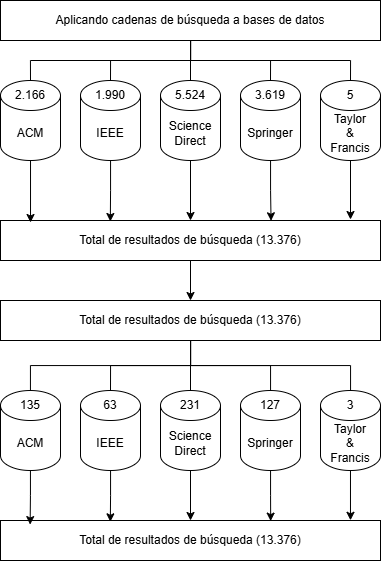
\includegraphics[scale=0.6] {tablas-images/sms/resumen_busqueda_bases.png}
	\caption{Diagrama resumen del proceso de búsqueda en bases de datos}\label{fig:resumen-busqueda-bases-de-datos}
\end{figure}




\section{Eliminación de duplicados}\label{sec:eliminacionDuplicados}
\noindent
La eliminación de estudios duplicados se efectuó mediante la herramienta de gestión bibliográfica Mendeley. Tras la recopilación inicial, todos los artículos fueron importados a dicha plataforma, la cual identificó y eliminó automáticamente las publicaciones redundantes. Este proceso resultó en la exclusión de \textbf{sesenta y tres} artículos duplicados, reduciendo el total de estudio a 496. La figura \ref{fig:eliminacion-duplicados} presenta una visualización gráfica de estos resultados.


% FIGURA Eliminación de duplicados
\begin{figure}[H]
	\centering
	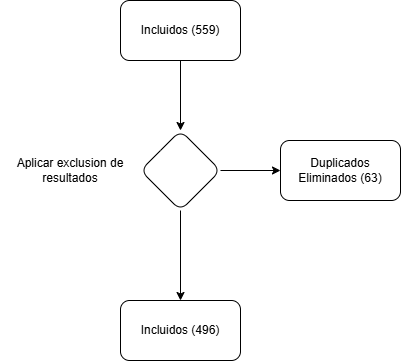
\includegraphics[scale=0.25] {tablas-images/sms/eliminacion-duplicados.png}
	\caption{Diagrama del proceso de eliminación de resultados}\label{fig:eliminacion-duplicados}
\end{figure}


\section{Priorización de estudios}\label{sec:priorizacionEstudios}
\noindent


Luego de la selección inicial de los artículos, se procedió a examinar los campos  \textit{title}, \textit{abstract} y \textit{keywords} de cada uno. Como resultado de esta revisión se generaron métricas de calidad para cada artículo, con el fin de priorizar aquellos más relevantes para la investigación. Las métricas utilizadas fueron las siguientes:

\begin{itemize}
	\item \textbf{SCI} \textit{(Science Citation Index)}
	\item \textbf{CVI} \textit{(Core Value Index)}
	\item \textbf{IRRQ} \textit{(Index Relation Research Question)}
\end{itemize}
\noindent

Este proceso inició con un total de 496 artículos, los cuales fueron evaluados según su alineamiento con los objetivos de la investigación. La evaluación temática permitió identificar un total de 68 artículos con una relación directa con el enfoque planteado.

\section{Estrategia de búsqueda usando bola de nieve}\label{sec:bolaDeNieve}
\noindent

En esta etapa, se seleccionaron los artículos cuya evaluación~\SCI~es alta, obteniendo un total de 15 artículos que constituyeron la línea base para el proceso de búsqueda por bola de nieve. A partir de esta base, se aplicó la estrategia de bola de nieve en ambas direcciones: hacia adelante (revisando referencias citadas por los artículos base) y hacia atrás (identificando artículos que citan a los de la base). Esta estrategia permitio la inclusion de cuarenta y dos estudios mediante la técnica hacia adelante y veintiún estudios mediante la técnica hacia adelante. En total, el proceso de bola de nieve generó 63 artículos adicionales. Sumando estos resultados a los 68 artículos previamente filtrados por \SCI, se obtuvo un corpus final de 131 artículos para el análisis.

El resumen de este proceso puede verse en la figura \ref{fig:resumen-snowball}

\begin{figure}[H]
	\begin{center}
		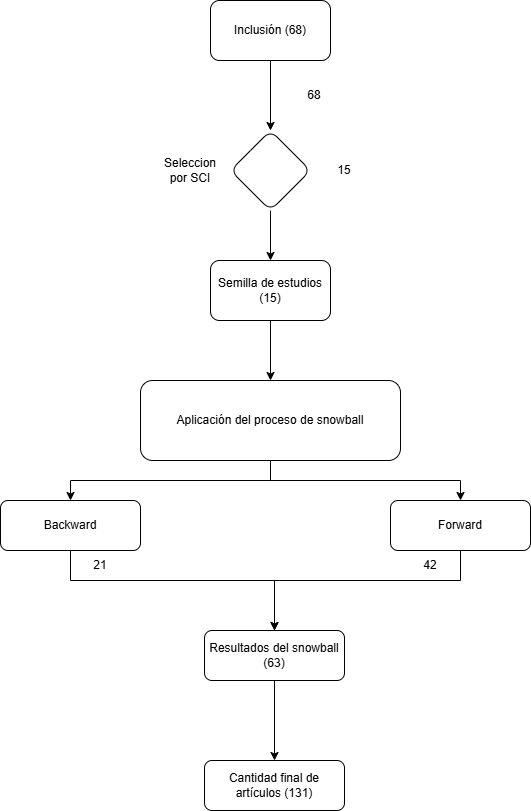
\includegraphics[width=0.6\textwidth]{tablas-images/sms/resumen-snowball.png}
	\end{center}
	\caption{Resumen del proceso de búsqueda por bola de nieve}\label{fig:resumen-snowball}
\end{figure}


\section{Identificación de estudios}

\section{Cuadro de estudios}

Los estudios resultantes del proceso de \SMS se presentan en la tabla \ref{table:selected_primary_studies}.



% -------- Tabla : Estudios Primarios Seleccionados (SPSs) ------------
\begin{table}[H]
	\centering
	\caption{Los 131 estudios primarios seleccionados (SPSs)}
	\label{table:selected_primary_studies}
	\fontsize{8pt}{10pt}\selectfont % Tamaño de fuente 8pt
	\renewcommand{\arraystretch}{1.2}
	\begin{tabular*}{\textwidth}{l @{\extracolsep{\fill}} r l @{\extracolsep{\fill}} r l @{\extracolsep{\fill}} r l @{\extracolsep{\fill}} r l @{\extracolsep{\fill}} r}
		\toprule
		\textbf{ID} & \textbf{Ref}                        & \textbf{ID} & \textbf{Ref}                        & \textbf{ID} & \textbf{Ref}                      & \textbf{ID} & \textbf{Ref}                        & \textbf{ID} & \textbf{Ref}                       \\
		\midrule
		SPS001      & \spsone                             & SPS002      & \spstwo                             & SPS003      & \spsthree                         & SPS004      & \spsfour                            & SPS005      & \spsfive                           \\
		SPS006      & \spssix                             & SPS007      & \spsseven                           & SPS008      & \spseight                         & SPS009      & \spsnine                            & SPS010      & \spsten                            \\
		SPS011      & \spseleven                          & SPS012      & \spstwelve                          & SPS013      & \spsthirteen                      & SPS014      & \spsfourteen                        & SPS015      & \spsfifteen                        \\
		SPS016      & \spssixteen                         & SPS017      & \spsseventeen                       & SPS018      & \spseighteen                      & SPS019      & \spsnineteen                        & SPS020      & \spstwenty                         \\
		SPS021      & \spstwentyone                       & SPS022      & \spstwentytwo                       & SPS023      & \spstwentythree                   & SPS024      & \spstwentyfour                      & SPS025      & \spstwentyfive                     \\
		SPS026      & \spstwentysix                       & SPS027      & \spstwentyseven                     & SPS028      & \spstwentyeight                   & SPS029      & \spstwentynine                      & SPS030      & \spsthirty                         \\
		SPS031      & \spsthirtyone                       & SPS032      & \spsthirtytwo                       & SPS033      & \spsthirtythree                   & SPS034      & \spsthirtyfour                      & SPS035      & \spsthirtyfive                     \\
		SPS036      & \spsthirtysix                       & SPS037      & \spsthirtyseven                     & SPS038      & \spsthirtyeight                   & SPS039      & \spsthirtynine                      & SPS040      & \spsforty                          \\
		SPS041      & \spsfortyone                        & SPS042      & \spsfortytwo                        & SPS043      & \spsfortythree                    & SPS044      & \spsfortyfour                       & SPS045      & \spsfortyfive                      \\
		SPS046      & \spsfortysix                        & SPS047      & \spsfortyseven                      & SPS048      & \spsfortyeight                    & SPS049      & \spsfortynine                       & SPS050      & \spsfifty                          \\
		SPS051      & \spsfiftyone                        & SPS052      & \spsfiftytwo                        & SPS053      & \spsfiftythree                    & SPS054      & \spsfiftyfour                       & SPS055      & \spsfiftyfive                      \\
		SPS056      & \spsfiftysix                        & SPS057      & \spsfiftyseven                      & SPS058      & \spsfiftyeight                    & SPS059      & \spsfiftynine                       & SPS060      & \spssixty                          \\
		SPS061      & \spssixtyone                        & SPS062      & \spssixtytwo                        & SPS063      & \spssixtythree                    & SPS064      & \spssixtyfour                       & SPS065      & \spssixtyfive                      \\
		SPS066      & \spssixtysix                        & SPS067      & \spssixtyseven                      & SPS068      & \spsixtyeight                     & SPS069      & \spssixtynine                       & SPS070      & \spsseventy                        \\
		SPS071      & \spsseventyone                      & SPS072      & \spsseventytwo                      & SPS073      & \spsseventythree                  & SPS074      & \spsseventyfour                     & SPS075      & \spsseventyfive                    \\
		SPS076      & \spsseventysix                      & SPS077      & \spsseventyseven                    & SPS078      & \spsseventyeight                  & SPS079      & \spsseventynine                     & SPS080      & \spseighty                         \\
		SPS081      & \spseightyone                       & SPS082      & \spseightytwo                       & SPS083      & \spseightythree                   & SPS084      & \spseightyfour                      & SPS085      & \spseightyfive                     \\
		SPS086      & \spseightysix                       & SPS087      & \spseightyseven                     & SPS088      & \spseightyeight                   & SPS089      & \spseightynine                      & SPS090      & \spsninety                         \\
		SPS091      & \spsninetyone                       & SPS092      & \spsninetytwo                       & SPS093      & \spsninetythree                   & SPS094      & \spsninetyfour                      & SPS095      & \spsninetyfive                     \\
		SPS096      & \spsninetysix                       & SPS097      & \spsninetyseven                     & SPS098      & \spsnineyeight                    & SPS099      & \spsninetynine                      & SPS100      & \spsonehundred                     \\
		SPS101      & \spsonehundredone                   & SPS102      & \spsonehundredtwo                   & SPS103      & \spsonehundredthree               & SPS104      & \spsonehundredfour                  & SPS105      & \spsonehundredfive                 \\
		SPS106      & \spsonehundredsix                   & SPS107      & \spsonehundredseven                 & SPS108      & \spsonehundredeight               & SPS109      & \spsonehundrednine                  & SPS110      & \spsonehundredten                  \\
		SPS111      & \spsonehundredeleven                & SPS112      & \spsonehundredtwelve                & SPS113      & \spsonehundredthirteen            & SPS114      & \spsonehundredfourteen              & SPS115      & \spsonehundredfifteen              \\
		SPS116      & \spsonehundredsixteen               & SPS117      & \spsonehundredseventeen             & SPS118      & \spsonehundredeighteen            & SPS119      & \spsonehundrednineteen              & SPS120      & \spsonehundredtwenty               \\
		SPS121      & \spsonehundredtwentyone             & SPS122      & \spsonehundredtwentytwo             & SPS123      & \spsonehundredtwentythree         & SPS124      & \spsonehundredtwentyfour            & SPS125      & \spsonehundredtwentyfive           \\
		SPS126      & \spsonehundredtwentysix             & SPS127      & \spsonehundredtwentyseven           & SPS128      & \spsonehundredtwentyeight         & SPS129      & \spsonehundredtwentynine            & SPS130      & \spsonehundredthirty               \\
		SPS131      & \spsonehundredthirtyone             &             &                                     &             &                                   &             &                                     &             &                                   \\
		\bottomrule
	\end{tabular*}
	\vspace{5pt}
\end{table}

%  --------------------------------------------------------------


\subsection{Artículos por año y métricas}
\noindent
A continuación se presentan las gráficas de los resultados de la búsqueda. En la figura \ref{fig:plot-anios-vs-indices-calidad} se muestra la relación entre la cantidad de estudios por año y las métricas definidas en las sección \ref{sec:priorizacionEstudios}

\begin{figure}[H]
	\begin{center}
		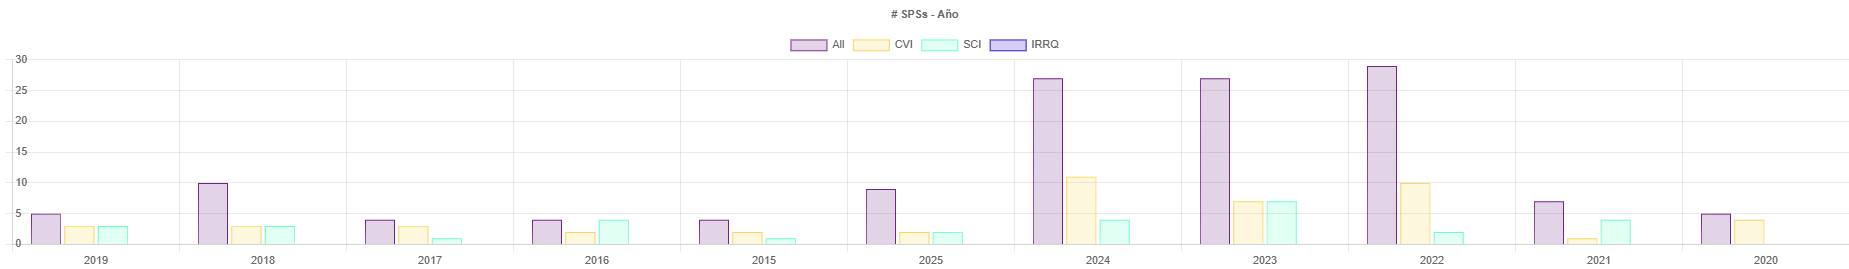
\includegraphics[width=0.95\textwidth]{tablas-images/sms/plot-freq-indices.png}
	\end{center}
	\caption{Cantidad de artículos en conformidad con las métricas de calidad definidas en \ref{sec:priorizacionEstudios}}
	\label{fig:plot-anios-vs-indices-calidad}
\end{figure}



\subsection{Diferencias entre estrategias}

En la figura \ref{fig:plot-estrategia_vs_articulos} se pude apreciar la cantidad de artículos obtenido por cada

\begin{figure}[H]
	\centering
	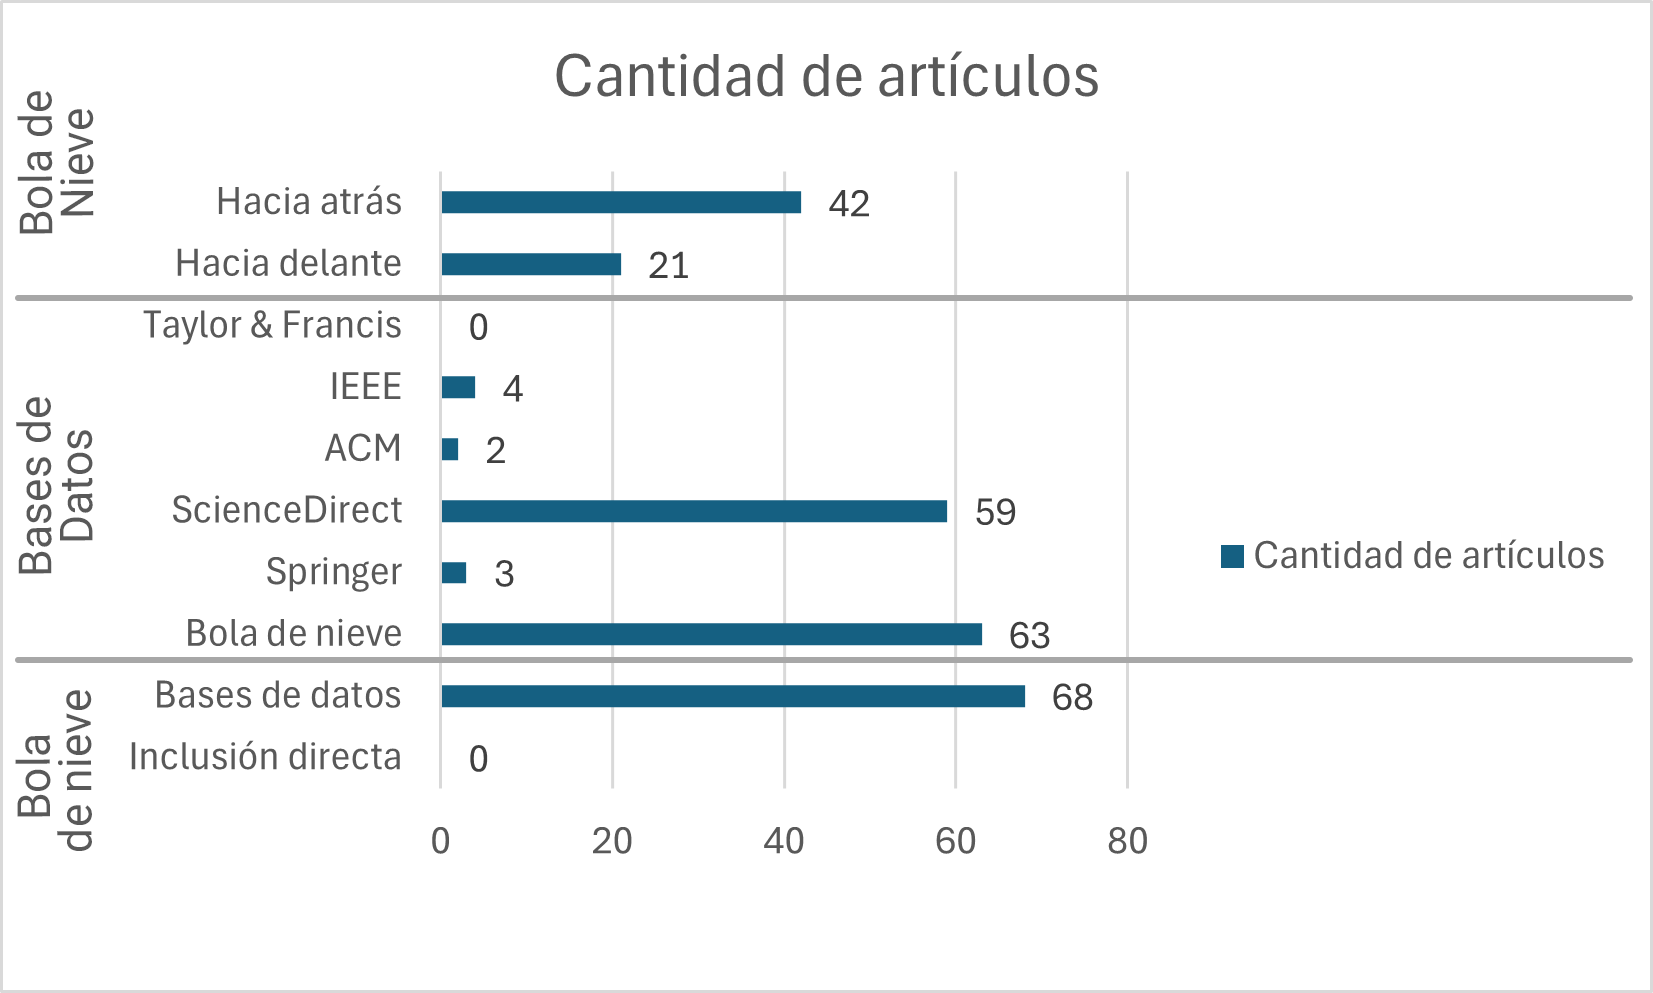
\includegraphics[scale=0.3] {tablas-images/sms/plot-estrategia_vs_articulos.png}
	\caption{Diagrama del proceso de eliminación de resultados}\label{fig:plot-estrategia_vs_articulos}
\end{figure}

\subsection{Tópicos frecuentes en los estudios}
\noindent

Del conjunto de 131 estudios analizados, se identificaron tópicos recurrentes mediante el análisis sistemático de los~\textit{abstracts} y~\textit{keywords} de cada publicación. Esta categorización temática reveló las áreas de investigación predominantes en el campo de estudio. Como se ilustra en la figura~\ref{fig:plot-topicos}, los tópicos más frecuentes incluyen \textbf{Model, \HPC, Methodology, \HTC, y Notation}, los cuales representan las tendencias principales en la literatura analizada.

\begin{figure}[H]
	\centering
	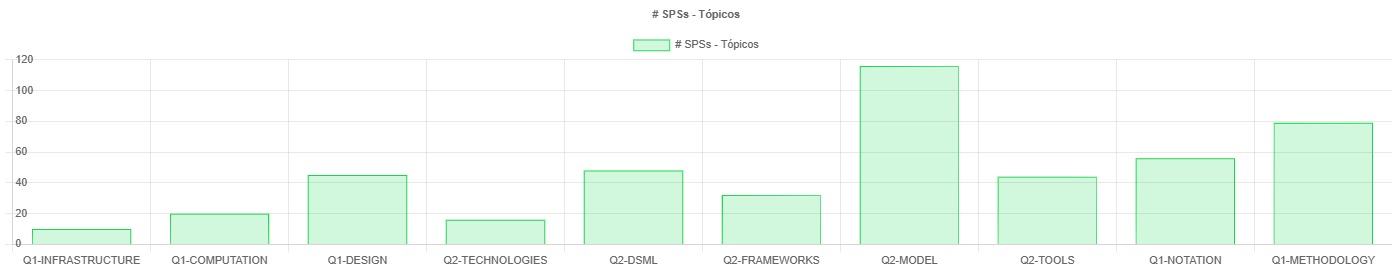
\includegraphics[scale=0.3] {tablas-images/sms/plot-topicos.png}
	\caption{Diagrama del proceso de eliminación de resultados}\label{fig:plot-topicos}
\end{figure}


\subsection{Conformidad con las preguntas de investigación}
Respecto al Cumplimiento con las preguntas de investigación (RQ) planteadas en la sección \ref{subsubsec:RQ-def}, 118 estudios cumplían con la \textbf{RQ1}, mientras que 130 de estos cumplían con la \textbf{RQ2}. Ver figura \ref{fig:plot-venn-RQs}

\begin{figure}[H]
	\centering
	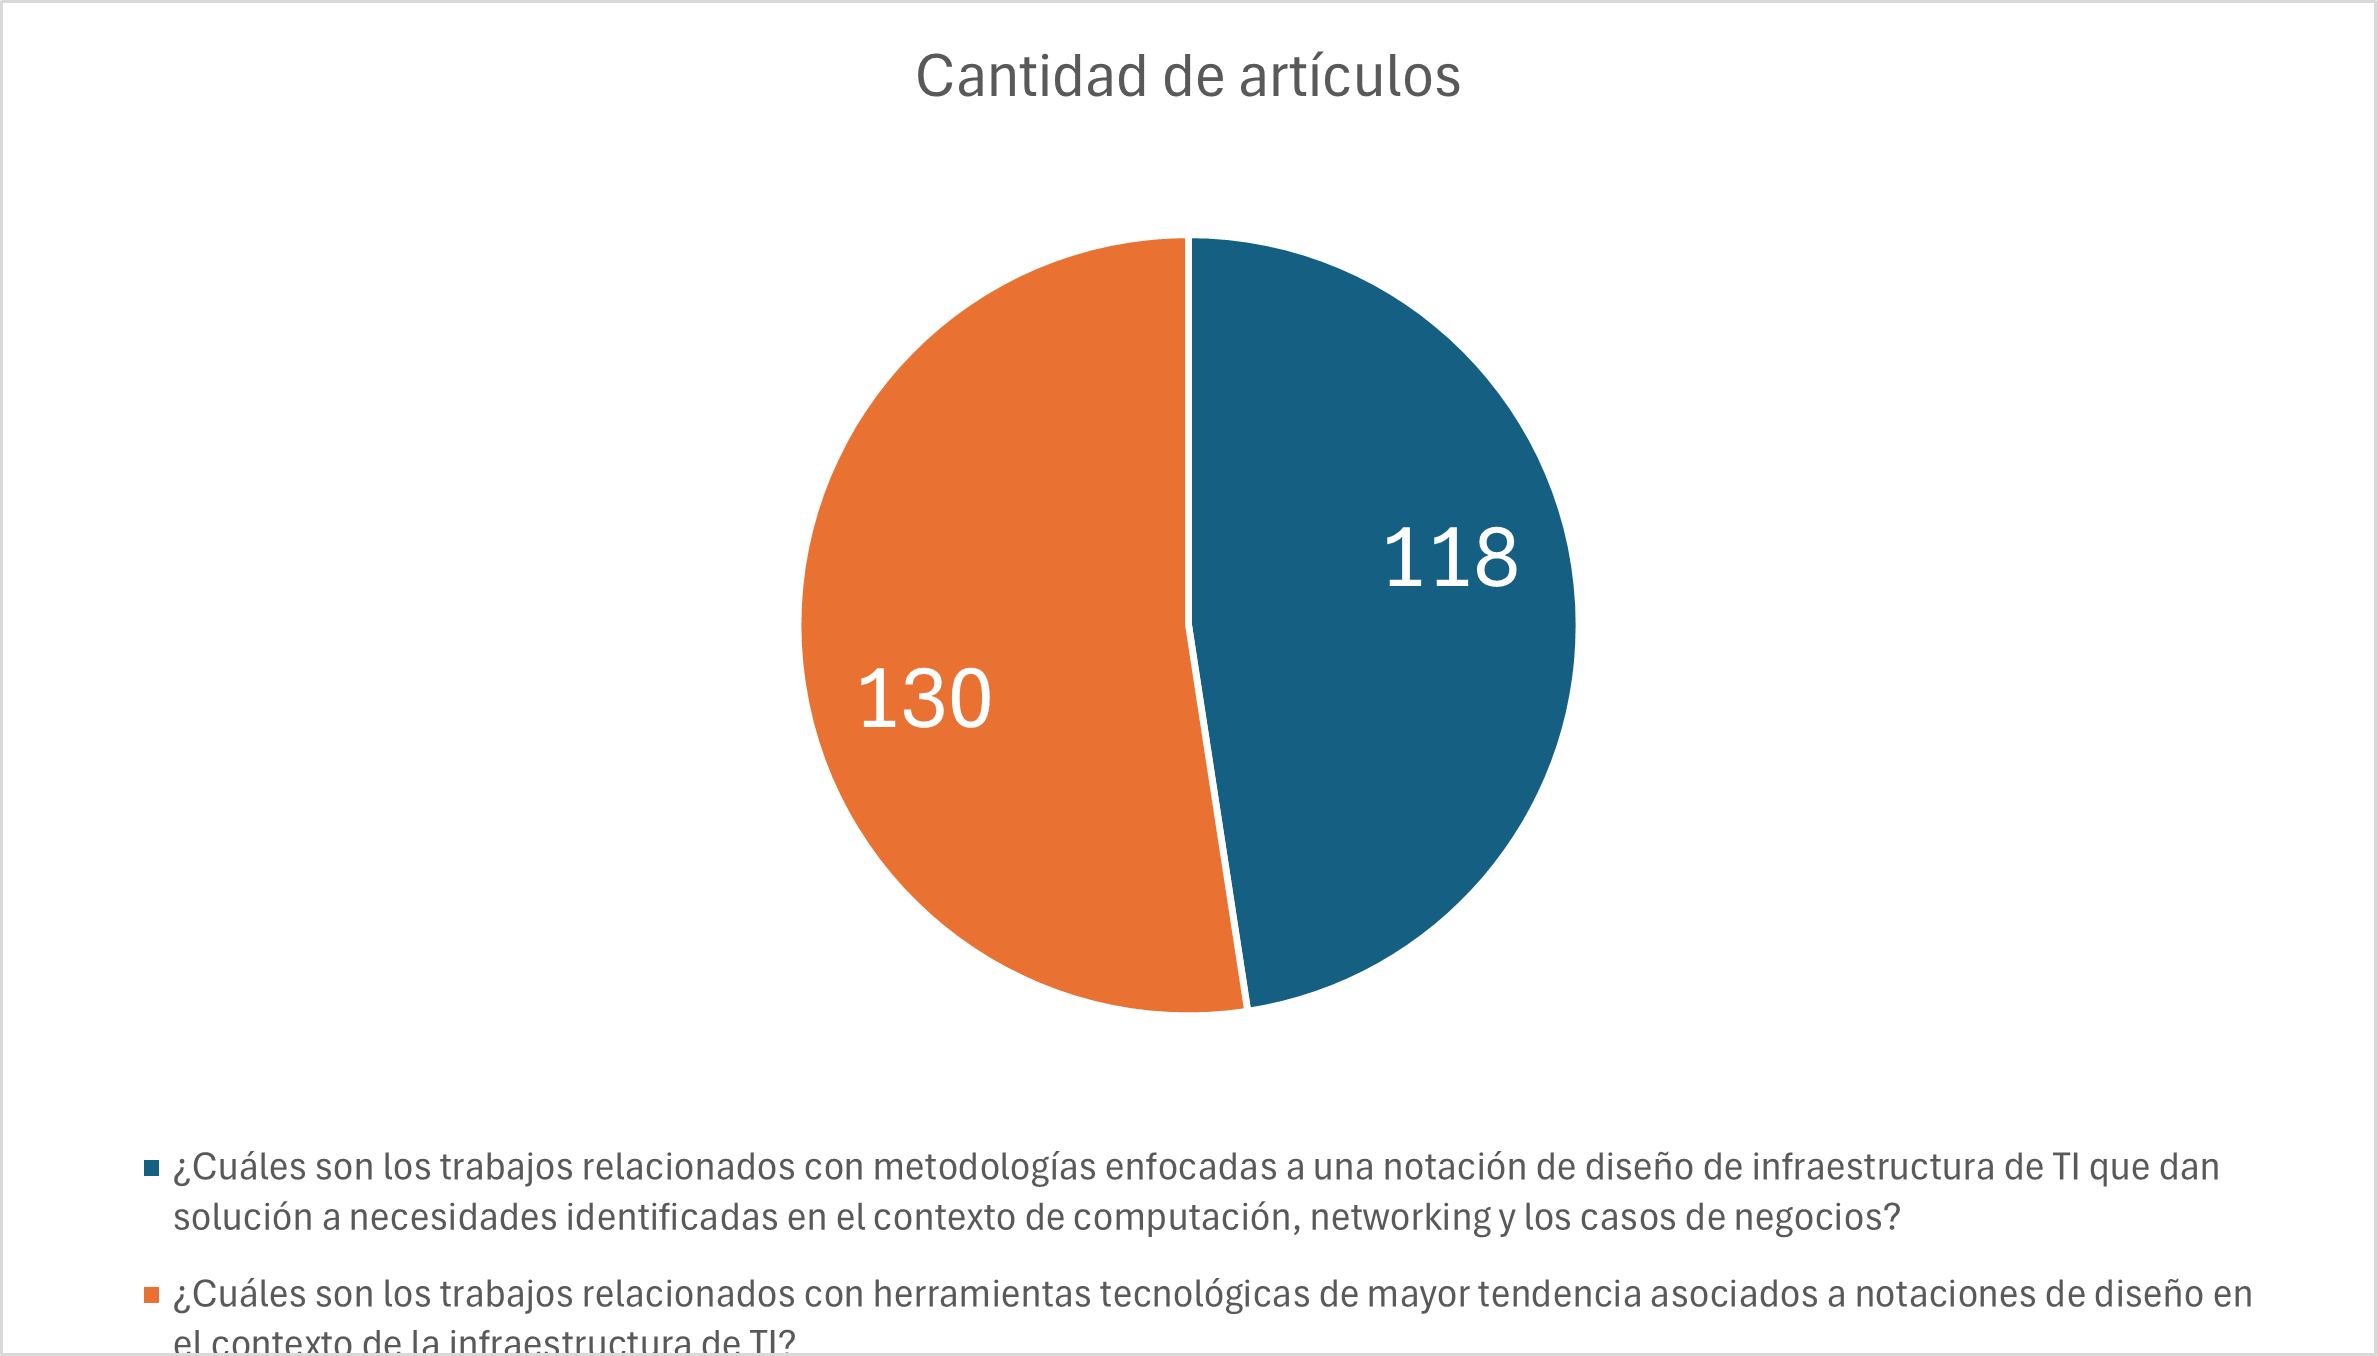
\includegraphics[scale=0.3] {tablas-images/sms/plot-venn-RQs.png}
	\caption{Diagrama del proceso de eliminación de resultados}\label{fig:plot-venn-RQs}
\end{figure}


\subsection{Taxonomía}

Con base en los resultados obetenidos hasta ahora en el proceso \SMS se consideró oportuno la construcción de un taxonomía que ayudase a clasificar aquellos topicos frecuentes encontrados en la literatura alrededor de las notaciones de diseño de infraestructura de TI. Dicha taxonomía se puede ver en la figura \ref{fig:taxonomia}

\begin{figure}[H]
	\centering
	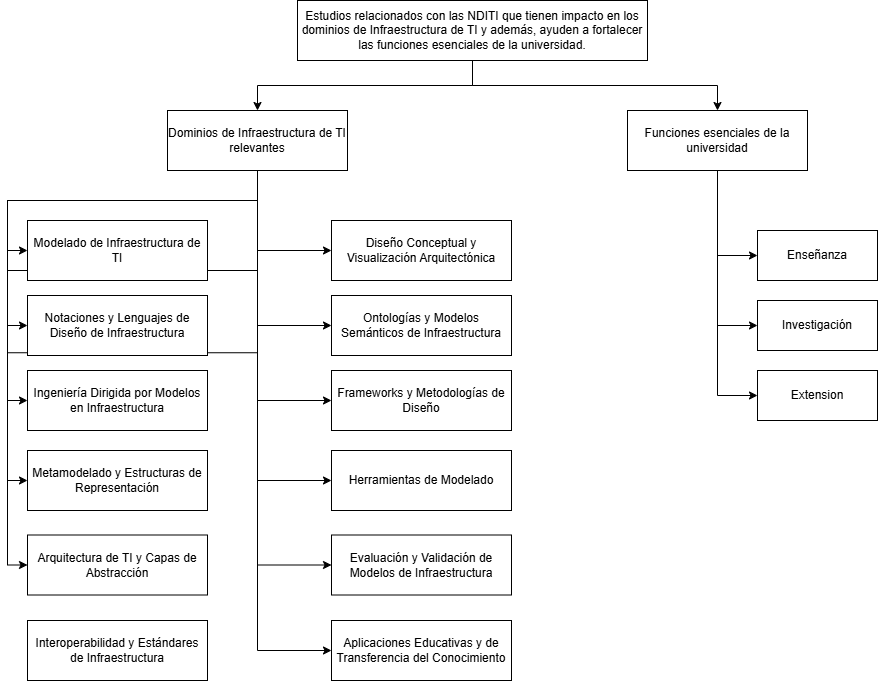
\includegraphics[scale=0.15] {tablas-images/sms/taxonomia.png}
	\caption{Taxonomía de los tópicos identificados en el \SMS}\label{fig:taxonomia}
\end{figure}





\section{Información de la herramienta}

\noindent
La herramienta utilizada para este proceso de revisión de la literatura fue \textbf{SMS-BUILDER}, desarrollada por el Dr. Christian Andres Candela Uribe la cual se encuentra disponible en \textit{Docker Hub}. La imagen puede consultarse en el siguiente enlace:

\begin{center}
	\href{https://hub.docker.com/r/griduq/sms-builder}{\texttt{https://hub.docker.com/r/griduq/sms-builder}}
\end{center}



\section{Reproducibilidad del método}
\noindent
Con el fin de fomentar la reproducibilidad del método de revisión, se proporcionan dos mecanismos de verificación que permiten a los revisores y lectores acceder de forma transparente a la información utilizada, generada mediante la herramienta SMS-Builder de~\cite{SMSBuilder2020}
\begin{itemize}
	\item Un enlace de acceso público a la instancia de SMS-Builder que contiene todos los datos del proceso de revisión sistemática: \href{https://sms-htcondor.iti.grid.uniquindio.edu.co}{link}. Las credenciales de acceso son ``invitado'' tanto para el nombre de usuario como para la contraseña.
	\item Una imagen de Docker de acceso público que integra toda la documentación necesaria para crear un contenedor con los datos del proceso: \href{https://hub.docker.com/r/parritap/sms-htcondor-universes}{link}.
\end{itemize}

\noindent
Adicionalmente, se implementaron procesos de respaldo como medida de seguridad. Estos \textit{backups} fueron almacenados en ubicaciones diferentes, siguiendo la estrategia de respaldo \textbf{3--2--1}.



\section{Conclusiones de la revisión sistemática de la literatura}
\noindent
Esta revisión sistemática de la literatura sobre Notaciones de Diseño de infraestructura de TI logró identificar y analizar 131 estudios relevantes de un total inicial de 559 documentos recuperados de cinco bases de datos académicas principales. El proceso metodológico incluyó la aplicación de criterios de inclusión y exclusión que redujeron el corpus inicial en un 95.73\%, seguido de la eliminación de duplicados y la aplicación de estrategias complementarias como la búsqueda por bola de nieve. Los resultados revelan que la base de datos Science Direct fue la fuente más productiva con el 41.29\% de los artículos iniciales, mientras que Taylor \& Francis no proporcionaron casi contribuciones significativas con las cadenas de búsqueda empleadas, representando unicamente el 0.03\%. El análisis temático identificó como tópicos predominantes \textbf{Model, \HPC, Methodology, \HTC, y Notation}, evidenciando una concentración de la investigación en estas áreas específicas. Respecto al cumplimiento de las preguntas de investigación, 118 estudios seleccionados (90.07\%) respondieron a RQ1 (trabajos relacionados con metodologíasenfocatadas a una \NDITI), mientras que 130 estudios (99.23\%) abordaron RQ2 (Trabajos relacionados con herramientas tecnológicas de mayor tendencia), lo que sugiere un interes significativo en la literatura tanto sobre las metodologías como tecnologías que guardan relación con las~\NDITI~en diferentes contextos. La distribución temporal de las publicaciones y la diversidad de métricas de calidad aplicadas confirman la relevancia y actualidad del tema de investigación, proporcionando una base sólida para el desarrollo de taxonomías y marcos de trabajo en el dominio de infraestructura de TI.